\documentclass[a4paper,10pt]{article}
\usepackage[utf8]{inputenc}
\usepackage{polski}
\usepackage{graphicx}
\usepackage{listings}
\usepackage[usenames,dvipsnames]{color}
\addtolength{\hoffset}{-1cm}
\addtolength{\voffset}{-2cm}
\addtolength{\textwidth}{2cm}
\addtolength{\textheight}{3cm}
\usepackage{setspace}
\usepackage{indentfirst}
\usepackage{graphicx}
\lstset{
    language=Matlab,
    basicstyle=\scriptsize,
    aboveskip={1.5\baselineskip},
    columns=fixed,
    showstringspaces=false,
    extendedchars=true,
    breaklines=true,
    tabsize=4,
    prebreak = \raisebox{0ex}[0ex][0ex]{\ensuremath{\hookleftarrow}},
    frame=single,
    showtabs=false,
    showspaces=false,
    showstringspaces=false,
    identifierstyle=\ttfamily,
    keywordstyle=\color[rgb]{0,0,1},
    commentstyle=\color[rgb]{0.133,0.545,0.133},
    stringstyle=\color[rgb]{0.627,0.126,0.941},
    numbers=left,
    numberstyle=\tiny,
    stepnumber=1,
    numbersep=5pt,
    captionpos=b,
    escapeinside={\%*}{*)}
}

\def\figurename{Rys.}
\def\lstlistingname{Fun.}

\title{Informatyczne Systemy Sterowania \\ \large Ćwiczenie 5: Sterowanie szybkością transmisji w sieci komputerowej}

\author{Adam Jordanek 168139, Tomasz Klimek 168092}

\begin{document}
\maketitle
\section{Wstęp}\label{sec:wstęp}
\subsection{Cel ćwiczenia}
%TODO -- skopiowane!!!
Celem ćwiczenia jest symulacja działania wybranego systemu sterowania ruchem w sieci 
komputerowej. Rozpatrywanym problemem jest sterowanie szybkością transmisji. 
Problem ten może być rozpatrywany jako zagadnienie sterowania w systemie 
zamkniętym. 
Najważniejsze  c e l e   ć w i c z e n i a   są następujące: 
1. Poznanie problemu sterowania ruchem w sieci komputerowej jako przykładu 
sterowania systemem komputerowym. 
2. Nabycie umiejętności wykorzystania pakietu Matlab oraz Simulink do symulacji ww. 
systemu. 
\subsection{Plan badań} 
\begin{enumerate}
	\item Symulacja systemu sterowania szybkością transmisji.
	\item Dobór optymalnego regulatora.
\end{enumerate}
\section{Realizacja planu i wyniki}

%-------------------------------------------------------------------------------------
%                                ZADANIE 1
%-------------------------------------------------------------------------------------
\subsection{Symulacja systemu sterowania szybkością transmisji}

Systemem symulowanym w tym ćwiczeniu będzie system opisany w artykule "\textit{Complete Stability Region
Characterization for PI-AQM}" , czyli system sterujący ruchem w sieci komputerowej. Z powyższego artykułu dla sieci, w której $C$ - przepustowość sieci, $N$ - ilość otwartych sieci TCP, oraz $d$ - opóźnienie pakietów, uzyskaliśmy następującą transmitancję.

\begin{equation} \label{eqn:transO}
	K_{O}(s)={B \over (s + \alpha) (s + \beta)}e^{-sd}
\end{equation}

Gdzie $\alpha = {2N \over d^{2}C}$, $\beta = {1 \over d}$ i $B = {C^2 \over 2N}$.

Regulować system będziemy używając regulatorów z rodziny PID (dzięki uprzejmości prowadzącego zajęcia laboratoryjne tylko P i PID), które opisane są poniższą transmitancją.

\begin{equation} \label{eqn:transR}
	K_{R}(s) = k + {T_{i} \over s} + T_{d}s ,
\end{equation}

Aby zasymulować system w Simulinku musieliśmy wymnożyć mianownik transmitancji obiektu tak, aby można było przedstawić go w postaci 2 bloczków (\textit{Transfer Fnc} i \textit{Transport Delay}).

\begin{equation} \label{eqn:transO}
	K_{O}(s)={B \over s^{2} + (\alpha + \beta)s + \alpha \beta}e^{-sd}
\end{equation}

\newpage
Gotowy schemat służący nam do symulacji przedstawiony jest na poniższym obrazku.

\begin{figure}[!h]
    \centering
	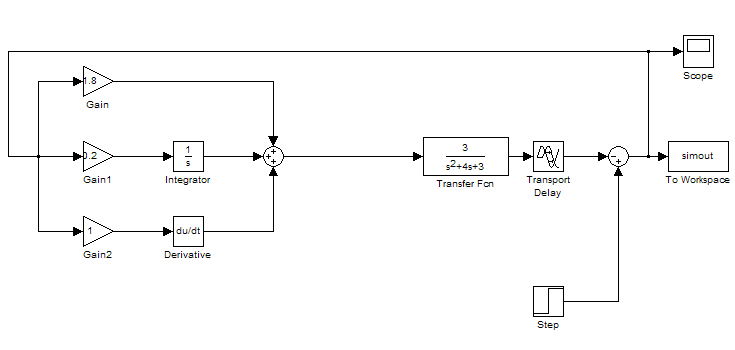
\includegraphics[width=120mm]{CW5-model-systemu.png}
	\caption{Schemat systemu służący nam do symulacji.}
    \label{fig:Rysunek}
\end{figure}

%-------------------------------------------------------------------------------------
%                                ZADANIE 2
%-------------------------------------------------------------------------------------
\subsection{Dobór optymalnego regulatora}

Przy doborze optymalnego regulatora i jego parametrów używaliśmy poniższej prostej funkcji napisanej w Matlabie.

%--------------
%zmieniłem trochę funkcję, żeby była czytelniejsza, z resztą i tak w większości wywoływałem ją dla 3:3,2:2, etc. ;)
%--------------
\begin{lstlisting}[caption=Funkcja testująca system.]
function test(N,C,r,p,i,d)
    load_system('PID.mdl');
    set_param('PID/Gain', 'Gain', num2str(p));   
    set_param('PID/Gain1', 'Gain', num2str(i));   
    set_param('PID/Gain2', 'Gain', num2str(d));
   
    set_param('PID/Transport Delay', 'DelayTime', num2str(r);        
        
    B=C(j+1)/2*N(j+1);
    set_param('PID/Transfer Fcn', 'Numerator', ['[',num2str(B),']']);        
        
    %Alfa i Beta 
    a=2*N/((r^2)*C);
    b=1/r;
    set_param('PID/Transfer Fcn', 'Denominator', ['[1 ',num2str(a+b),' ',num2str(a*b),']']);        
        
    sim('PID.mdl');
    wy = simout.signals.values;    
  	plot(tout, wy, '-k');
end
\end{lstlisting}

Aby zacząć testować system wybraliśmy parametry obiektu, dla których przeprowadzaliśmy dalsze testy, Mianowicie wybraliśmy $C = 3$, $N = 2$, $d = 1$

\newpage
\subsubsection{Regulator P}

Tutaj coś, że wywołujemy dla (C,N,d,p,0,0), żeby mieć regulator P, a potem parę wykresów żeby dobrać k...

\subsubsection{Regulator PID}

\section{Wnioski.}\label{sec:wnioski}

\end{document}